% ----- Page de Garde -----

\begin{center}
    
\includegraphics[width=0.35\textwidth]{image/ISEN.png}
\end{center}

\rule{\linewidth}{0.5mm}

\begin{center}
    \Huge \bf Final Project \\
    \LARGE \bf The Maximum Edge Weight Clique Problem
\end{center}

\rule{\linewidth}{0.5mm}

\vspace{1\baselineskip}

\begin{center}
    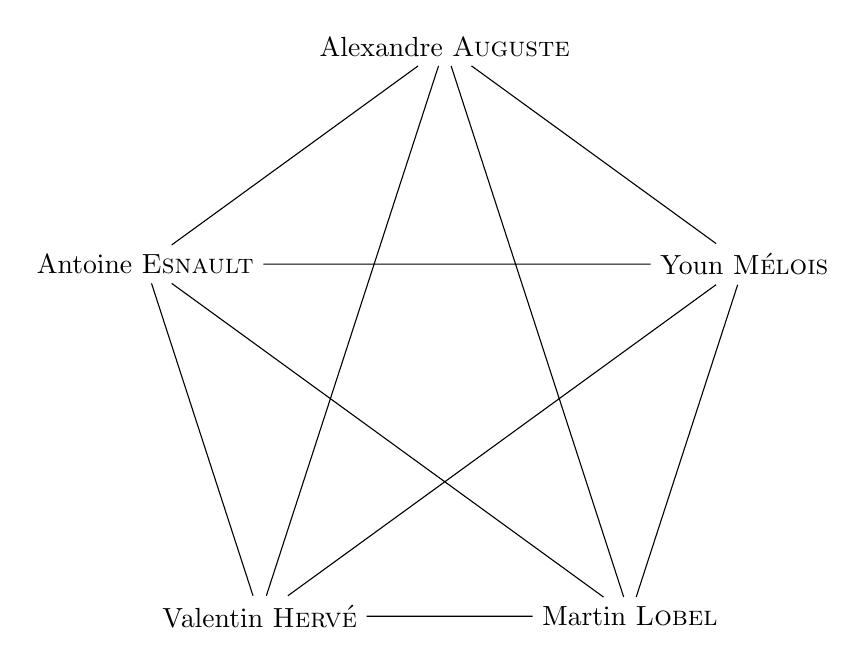
\begin{tikzpicture}[every text node part/.style={align=center}]
        \node (P0) at (90:4cm) {Alexandre \textsc{Auguste}};
        \node (P1) at (90+72:4cm) {Antoine \textsc{Esnault}};
        \node (P2) at (90+2*72:4cm) {Valentin \textsc{Herv\'e}};
        \node (P3) at (90+3*72:4cm) {Martin \textsc{Lobel}};
        \node (P4) at (90+4*72:4cm) {Youn \textsc{M\'elois}};

        \draw (P0)
        -- (P1)
        -- (P2)
        -- (P3)
        -- (P4)
        -- (P0)
        -- (P2)
        -- (P4)
        -- (P1)
        -- (P3)
        -- (P0);
    \end{tikzpicture}
\end{center}
\large\textbf{Abstract} \newline
The Maximum Edge Weight Clique (MEWC) problem is an optimization problem in
graph theory that asks for the clique (a subset of vertices, all adjacent to
one another) with the maximum total weight in an edge-weighted undirected graph.
In the MEWC problem, each edge has a weight, and the weight of a clique is the
sum of the weights of its edges. The goal is to find a clique with the maximum
possible weight.

\begin{center} \Large
    \emph{Class group:} \\
    CIR3 - Team 1
\end{center}

\begin{center} \Large
    \emph{Teacher:} \\
    Leandro \textsc{Montero}
\end{center}

\vfill

\begin{center} \Large
    \today
\end{center}

\newpage